

\documentclass{beamer}
\usetheme{Frankfurt}
\usecolortheme{dove}
\usepackage{graphicx}
\usepackage{xcolor}
\usepackage{multicol}
\newcommand\independent{\protect\mathpalette{\protect\independenT}{\perp}}
\newcommand\indep{\protect\mathpalette{\protect\independenT}{\perp}}
\def\independenT#1#2{\mathrel{\rlap{$#1#2$}\mkern2mu{#1#2}}}
\definecolor{dblue}{RGB}{0,0,139}
\usepackage{tikz}
\usetikzlibrary{arrows,shapes.arrows,positioning,shapes,shapes.misc}
\usetikzlibrary{decorations.pathreplacing}
\usepackage{booktabs}
\renewcommand{\arraystretch}{1.2}
\newcommand{\Cov}{\text{Cov}}
\newcommand{\Cor}{\text{Cor}}
\newcommand{\V}{\mathbb{V}}
\renewcommand{\P}{\mathbb{P}}
\newcommand{\E}{\mathbb{E}}
\newcommand{\doop}{\text{do}}
\usepackage{hanging}% http://ctan.org/pkg/hanging
\setbeamertemplate{footnote}{%
  \hangpara{2em}{1}%
  \makebox[2em][l]{\insertfootnotemark}\footnotesize\insertfootnotetext\par%
}
\newcommand{\myfootnote}{\let\thefootnote\relax\footnote}
\newcommand{\blue}[1]{\textcolor{blue}{#1}}
\newcommand{\gray}[1]{\textcolor{gray}{#1}}
\newcommand{\green}[1]{\textcolor{olive}{#1}}
\newcommand{\purple}[1]{\textcolor{purple}{#1}}
\newcommand{\bred}[1]{\textbf{\textcolor{red}{#1}}}
\newcommand{\bblue}[1]{\textbf{\textcolor{blue}{#1}}}
\newcommand{\bgreen}[1]{\textbf{\textcolor{olive}{#1}}}
\newcommand{\bpurple}[1]{\textbf{\textcolor{purple}{#1}}}
\newcommand\black[1]{\color{black}#1}
\newcommand\white[1]{\color{white}#1}
\usepackage{array}
\newcolumntype{L}[1]{>{\raggedright\let\newline\\\arraybackslash\hspace{0pt}}m{#1}}
\usepackage[round]{natbib}
\bibliographystyle{humannat-mod}
\setbeamertemplate{footnote}{%
  \footnotesize\insertfootnotetext\par%
}
\setbeamertemplate{enumerate items}[default]
\usepackage[append]{beamersubframe}
\title{Consistency}
\author{Ian Lundberg}
\institute[Princeton University] % (optional, but mostly needed)
{
  Department of Sociology and Office of Population Research\\
  Princeton University
}

\newcommand\mytc[3]{
\begin{frame}
\begin{center}
\large
\bblue{Versions of Treatment}\\A Causal Inference Debate Sociologists Have Ignored
\end{center}
\begin{tikzpicture}[y = .5cm]
\node[anchor = west] at (0,-1) {\hyperlink{sec:problem}{1. Formalizing the \bgreen{problem}}};
	\node[anchor = west, font = \small]  at (1, -2) {\hyperlink{sec:potentialOutcomes}{A) Potential outcomes}};
	\node[anchor = west, font = \small]  at (1, -3) {\hyperlink{sec:stochasticCounterfactuals}{B) Stochastic counterfactuals}};
	\node[anchor = west, font = \small]  at (1, -4) {\hyperlink{sec:causalGraphs}{C) Causal graphs}};
\node[anchor = west]  at (0,-5.5) {\hyperlink{sec:consequences}{2. When it matters: \bgreen{Consequences} of collapsed versions}};
	\node[anchor = west, font = \small]  at (1, -6.5) {\hyperlink{sec:experiments}{A) Experimental studies: Effects may not generalize}};
	\node[anchor = west, font = \small]  at (1, -7.5) {\hyperlink{sec:observational}{B) Observational studies:}};
	\node[anchor = west, font = \small] at (1.5, -8.5) {\hyperlink{sec:unusualAverage}{--- ``Effects'' may be an unusual average}};
	\node[anchor = west, font = \small] at (1.5, -9.5) {\hyperlink{sec:heterogeneousEffects}{--- Heterogeneous treatment effects may really be}};
	\node[anchor = west, font = \small] at (1.5, -10.5) {\hyperlink{sec:heterogeneousEffects}{\textcolor{white}{---} the effects of heterogeneous treatments}};
\node[anchor = west, font = \small] at (0, -12) {\hyperlink{sec:recommendations}{3. \bgreen{Recommendations:} What to do}};
% Arrow indicating where we are
\draw[->, #3, line width = 2pt] (-.5, #1) -- (#2, #1);
\end{tikzpicture}
\end{frame}
}

\newcommand\exampleSlideExperimental{
\begin{frame}{Generalizing experimental evidence}
\begin{tikzpicture}[x = .5\textwidth, y = .45\textheight]
\node at (-1,-1) {};
\node at (1,1) {};
%%%%%%%%%%
%%%%%%%%%%
\node[anchor = north, align = center] at (-.5,1) {Generalization \bred{impossible}};
\node (a1) at (-.85, .45) {$A$};
%\node (d1) at (-.5, .45) {$D$};
\node (x1) at (-.15, .65) {$U$};
\node (y1) at (-.15, .45) {$Y$};
\draw[->, thick] (a1) -- (y1);
%\draw[->, thick] (a1) -- (d1);
%\draw[->, thick] (d1) -- (y1);
\draw[->, thick] (x1) -- (y1);
\node[font = \footnotesize, align = center] (t1) at (-.85, .65) {Target\\population};
\draw[<->, thick] (t1.east) to[bend left = 20] (x1.west);
\node[anchor = north, align = center, font = \footnotesize] at (a1.south) {Push\\notification\\sent};
%\node[anchor = north, align = center, font = \footnotesize] at (d1.south) {iPhone push\\Android push\\No push};
\node[anchor = north, align = center, font = \footnotesize] at (y1.south) {Health};
%%%%%%%%%%
%%%%%%%%%%
\node[anchor = north, align = center] at (.5,1) {Generalization \bblue{possible}\\by randomizing $D$};
\node (a2) at (.15, .45) {$A$};
\node (d2) at (.5, .45) {$D$};
\node (x2) at (.5, .65) {$U$};
\node (y2) at (.85, .45) {$Y$};
\draw[->, thick] (a2) -- (d2);
\draw[->, thick] (d2) -- (y2);
\draw[->, thick] (x2) -- (d2);
\node[font = \footnotesize, align = center] (t2) at (.15, .65) {Target\\population};
\draw[<->, thick] (t2.east) to[bend left = 20] (x2.west);
\node[anchor = north, align = center, font = \footnotesize] at (a2.south) {Push\\notification\\sent};
\node[anchor = north, align = center, font = \footnotesize] at (d2.south) {iPhone push\\Android push\\No push};
\node[anchor = north, align = center, font = \footnotesize] at (y2.south) {Health};
%%%%%%%%%%
%%%%%%%%%%
\node[anchor = north, align = center] at (-.5,0) {Generalization \bred{impossible}};
\node (a3) at (-.85, -.55) {$A$};
\node (d3) at (-.5, -.55) {$D$};
\node (x3) at (-.5, -.35) {$X$};
\node (u3) at (-.15, -.35) {$U$};
\node (y3) at (-.15, -.55) {$Y$};
\draw[->, thick] (a3) -- (d3);
\draw[->, thick] (d3) -- (y3);
\draw[->, thick] (x3) -- (d3);
\draw[->, thick] (u3) -- (x3);
\draw[->, thick] (u3) -- (y3);
\node[font = \footnotesize, align = center] (t3) at (-.85, -.35) {Target\\population};
\draw[<->, thick] (t3.east) to[bend left] (x3.west);
\node[anchor = north, align = center, font = \footnotesize] at (a3.south) {Push\\notification\\sent};
%\node[anchor = west, align = center, font = \footnotesize] at (x3.east) {Phone type};
\node[anchor = north, align = center, font = \footnotesize] at (d3.south) {iPhone push\\Android push\\No push};
\node[anchor = north, align = center, font = \footnotesize] at (y3.south) {Health};
%%%%%%%%%%
%%%%%%%%%%
\node[anchor = north, align = center] at (.5,0) {Generalization \bblue{possible}\\{\footnotesize by randomizing $D$ and observing $X$}};
\node (a4) at (.15, -.55) {$A$};
\node (d4) at (.5, -.55) {$D$};
\node (u4) at (.5, -.35) {$U$};
\node (x4) at (.85, -.35) {$X$};
\node (y4) at (.85, -.55) {$Y$};
\draw[->, thick] (a4) -- (d4);
\draw[->, thick] (d4) -- (y4);
\draw[->, thick] (x4) -- (y4);
\draw[->, thick] (x4) -- (u4);
\draw[->, thick] (u4) -- (d4);
\node[font = \footnotesize, align = center] (t4) at (.15, -.35) {Target\\population};
\draw[<->, thick] (t4.east) to[bend left = 15] (u4.west);
\draw[<->, thick] (t4.east) to[bend left = 15] (x4.north west);
\node[anchor = north, align = center, font = \footnotesize] at (a4.south) {Push\\notification\\sent};
%\node[anchor = west, align = center, font = \footnotesize] at (x4.east) {Phone type};
\node[anchor = north, align = center, font = \footnotesize] at (d4.south) {iPhone push\\Android push\\No push};
\node[anchor = north, align = center, font = \footnotesize] at (y4.south) {Health};
\end{tikzpicture}
\end{frame}
}

\newcommand\exampleSlide{
\begin{frame}{Four observational examples}
\begin{tikzpicture}[x = .5\textwidth, y = .45\textheight]
\node at (-1,-1) {};
\node at (1,1) {};
%%%%%%%%%%
%%%%%%%%%%
\node[anchor = north, align = center] at (-.5,1) {\bblue{Overwork}\\{\small Researcher collapses continuous $D$}};
\node (d4) at (-.7, .45) {$D$};
\node (y4) at (-.3, .45) {$Y$};
\node (a4) at (-.5, .65) {$A = \mathcal{C}(D) = \mathbb{I}(D>50)$};
\draw[->, thick] (d4) -- (y4);
\node[anchor = north, align = center, font = \footnotesize] at (d4.south) {Employment\\hours};
\node[anchor = north, align = center, font = \footnotesize] at (y4.south) {Hourly\\wage};
%%%%%%%%%%
%%%%%%%%%%
\node[anchor = north, align = center] at (.5,1) {\bblue{Occupations}\\{\small Researcher collapses categorical $D$}};
\node (d3) at (.3, .45) {$D$};
\node (y3) at (.7, .45) {$Y$};
\node (a3) at (.5, .65) {Class scheme: $A = \mathcal{C}(D)$};
\draw[->, thick] (d3) -- (y3);
\node[anchor = north, align = center, font = \footnotesize] at (d3.south) {Occupation};
\node[anchor = north, align = center, font = \footnotesize] at (y3.south) {Status};
%%%%%%%%%%
%%%%%%%%%%
\node[anchor = north, align = center] at (-.5,0) {\bblue{Attachment to school}\\{\small Respondent collapses continuous $D$}};
\node (d2) at (-.7, -.55) {$D$};
\node (y2) at (-.3, -.55) {$Y$};
\node (a2) at (-.5, -.35) {5-point scale: $A = \mathcal{C}(D)$};
\draw[->, thick] (d2) -- (y2);
\node[anchor = north, align = center, font = \footnotesize] at (d2.south) {Attachment\\to school};
\node[anchor = north, align = center, font = \footnotesize] at (y2.south) {Achievement};
%%%%%%%%%%
%%%%%%%%%%
\node[anchor = north, align = center] at (.5,0) {\bblue{Mobile health}\\{\small Generalizing experimental estimates}};
\node (a1) at (.1, -.55) {$A$};
\node (d1) at (.5, -.55) {$D$};
\node (x1) at (.5, -.35) {User platform};
\node (y1) at (.9, -.55) {$Y$};
\draw[->, thick] (a1) -- (d1);
\draw[->, thick] (d1) -- (y1);
\draw[->, thick] (x1) -- (d1);
\node[anchor = north, align = center, font = \footnotesize] at (a1.south) {Push\\notification\\sent};
\node[anchor = north, align = center, font = \footnotesize] at (d1.south) {iPhone push\\Android push\\No push};%{Delivery\\platform};
\node[anchor = north, align = center, font = \footnotesize] at (y1.south) {Health};
\end{tikzpicture}
\end{frame}
}

\newcommand\exampleSlideObservational[1]{
\begin{frame}
\begin{tikzpicture}[x = .5\textwidth, y = .45\textheight]
\node at (-1,-1) {};
\node at (1,1) {};
\node[rotate = 90, gray,align=center] at (-1.02,.5) {Collapsed by\\\textbf{researcher}};
\node[rotate = 90, gray,align=center] at (-1.02,-.5) {Collapsed by\\\textbf{respondent}};
\node[anchor = south, gray] at (-.5,1) {\textbf{Continuous} treatment};
\node[anchor = south, gray] at (.5,1) {\textbf{Categorical} treatment};
\draw[thick, gray] (0,1.05) -- (0,-1);
\draw[thick, gray] (-1.05,0.03) -- (1,0.03);
%%%%%%%%%%
%%%%%%%%%%
\node[anchor = north, align = center] at (-.5,1) {\bblue{Overwork}\\{\footnotesize Researcher collapses continuous $D$}};
\node (d4) at (-.7, .45) {$D$};
\node (y4) at (-.3, .45) {$Y$};
\node (a4) at (-.5, .65) {$A = \mathcal{C}(D) = \mathbb{I}(D>50)$};
\draw[->, thick] (d4) -- (y4);
\node[anchor = north, align = center, font = \footnotesize] at (d4.south) {Employment\\hours};
\node[anchor = north, align = center, font = \footnotesize] at (y4.south) {Hourly\\wage};
%%%%%%%%%%
%%%%%%%%%%
\node[anchor = north, align = center] at (.5,1) {\bblue{Occupations}\\{\footnotesize Researcher collapses categorical $D$}};
\node (d3) at (.3, .45) {$D$};
\node (y3) at (.7, .45) {$Y$};
\node (a3) at (.5, .65) {Class scheme: $A = \mathcal{C}(D)$};
\draw[->, thick] (d3) -- (y3);
\node[anchor = north, align = center, font = \footnotesize] at (d3.south) {Occupation};
\node[anchor = north, align = center, font = \footnotesize] at (y3.south) {Status};
%%%%%%%%%%
%%%%%%%%%%
\node[anchor = north, align = center] at (-.5,0) {\bblue{Self-rated health}\\{\footnotesize Respondent collapses continuous $D$}};
\node (d2) at (-.7, -.55) {$D$};
\node (y2) at (-.3, -.55) {$Y$};
\node (a2) at (-.5, -.35) {5-point scale: $A = \mathcal{C}(D)$};
\draw[->, thick] (d2) -- (y2);
\node[anchor = north, align = center, font = \footnotesize] at (d2.south) {Health};
\node[anchor = north, align = center, font = \footnotesize] at (y2.south) {Lifespan};
%%%%%%%%%%
%%%%%%%%%%
\node[anchor = north, align = center] at (.5,0) {\bblue{Returns to college}\\{\footnotesize Respondent collapses categorical $D$}};
\node (d4) at (.3, -.55) {$D$};
\node (y4) at (.7, -.55) {$Y$};
\node (a4) at (.5, -.35) {Completed college: $A = \mathcal{C}(D)$};
\draw[->, thick] (d4) -- (y4);
\node[anchor = north, align = center, font = \footnotesize] at (d4.south) {College degree\\(institution\\and major)};
\node[anchor = north, align = center, font = \footnotesize] at (y4.south) {Earnings};
#1
\end{tikzpicture}
\end{frame}
}

\date{\today}

\begin{document}

\begin{frame}
\centering
\begin{huge}
\textcolor{blue}{Versions of Treatment}\vskip .1cm 
\end{huge} \begin{Large}
A causal inference debate that\\sociologists have ignored
\end{Large}\vskip .2cm
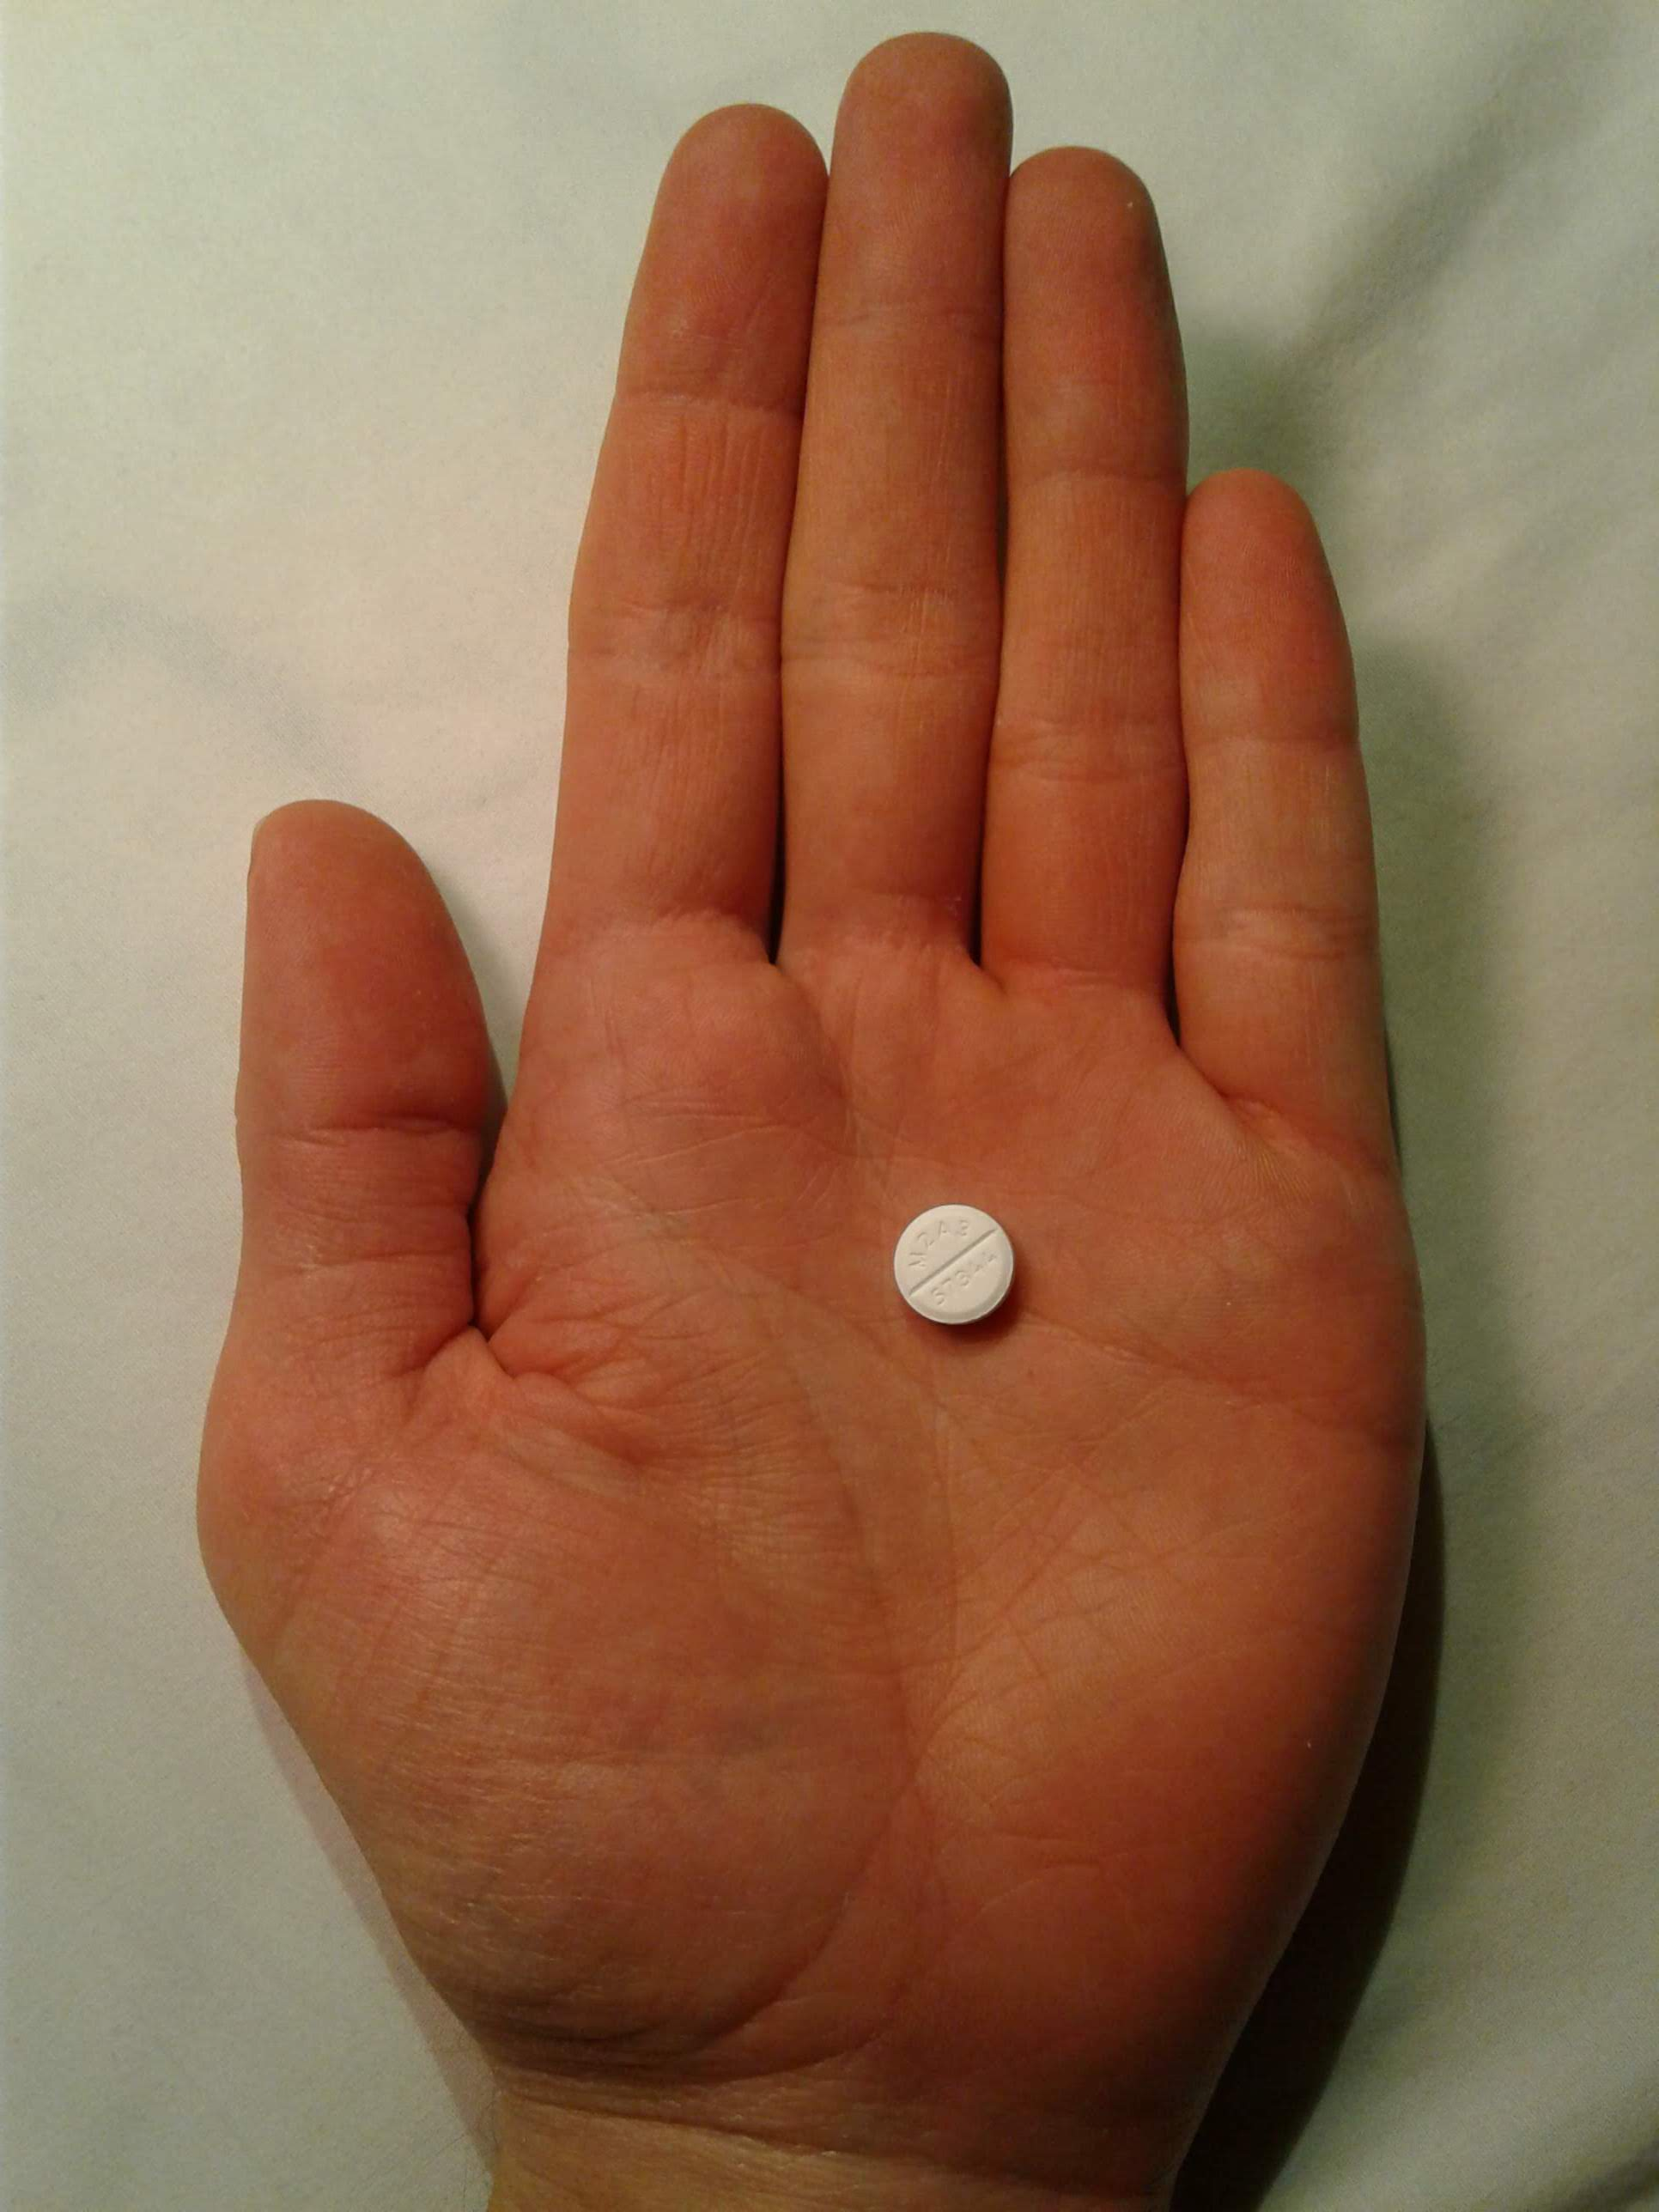
\includegraphics[width = .25\textwidth]{figures/left_hand}\hspace{20pt}
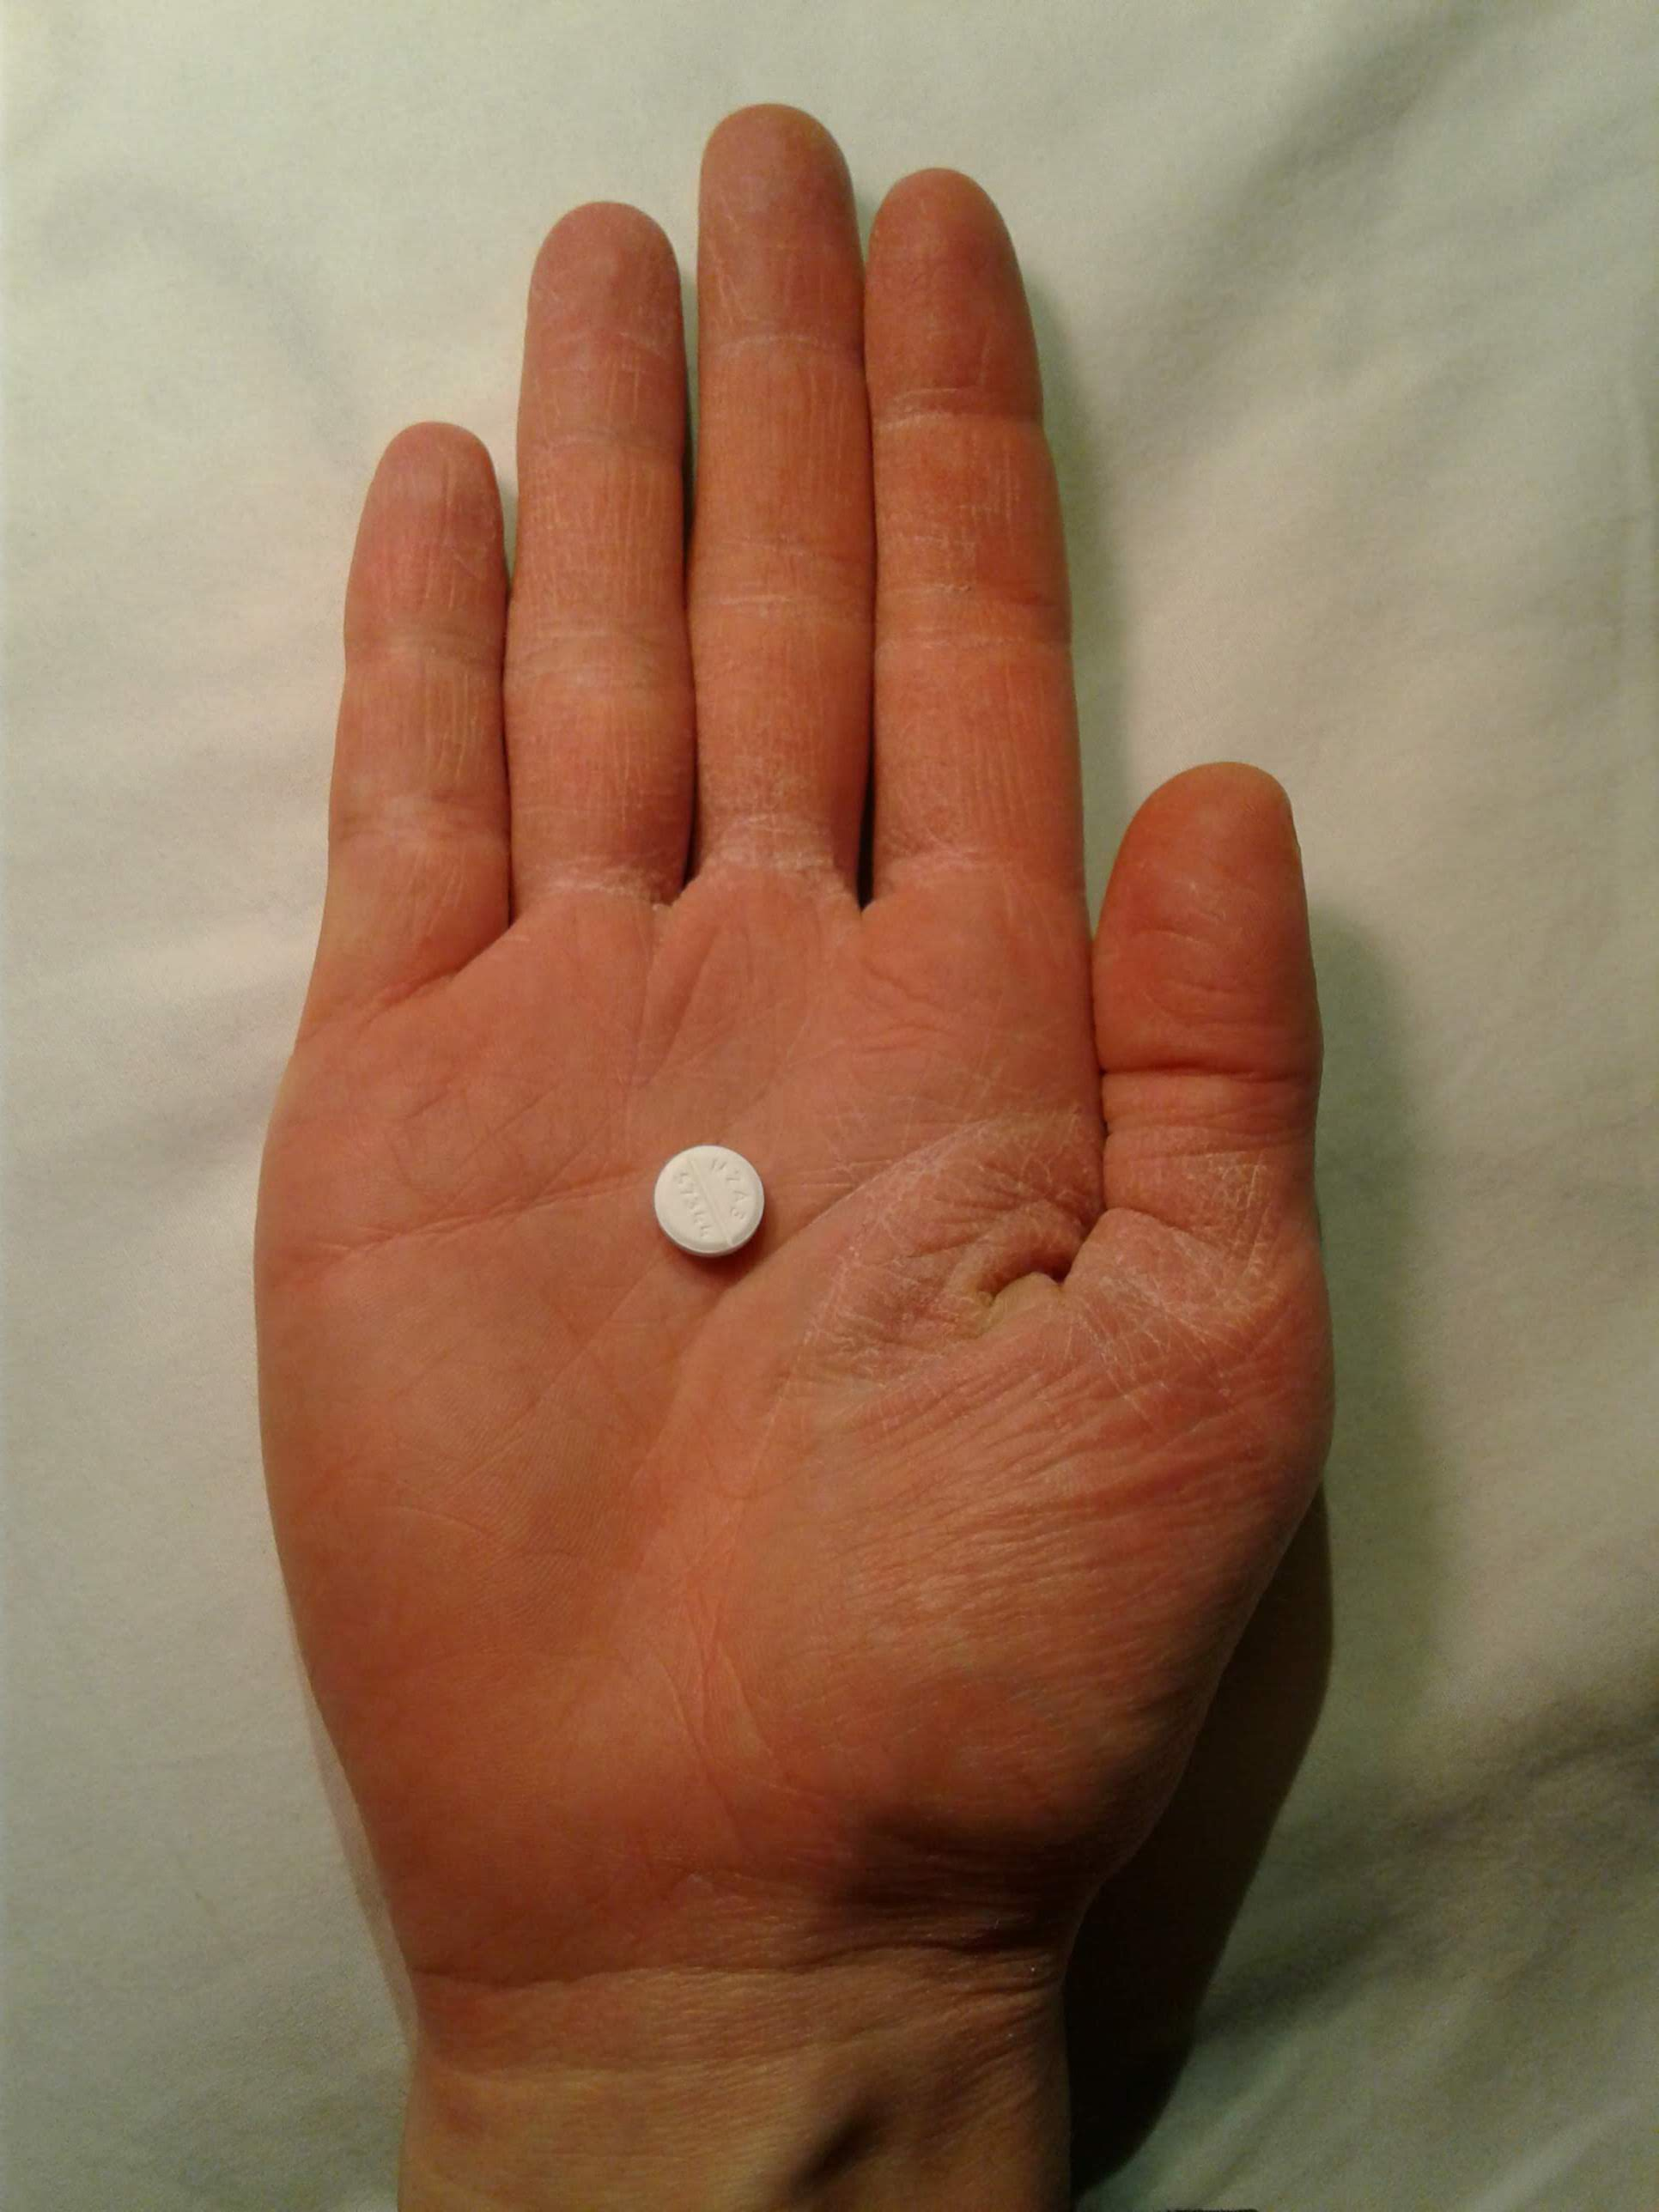
\includegraphics[width = .25\textwidth]{figures/right_hand} \vskip .2cm
Ian Lundberg \\
Princeton University \\
Sociology Statistics Reading Group\\
20 February 2019
\end{frame}

\begin{frame}{Introductory note for those finding these slides online}
These slides were prepared for the \href{https://scholar.princeton.edu/bstewart/sociology-statistics-reading-group}{Sociology Statistics Reading Group} at Princeton. Everyone read the following paper in advance:
\begin{quote}\normalfont
Hern\'an, Miguel A. 2016. Does water kill? A call for less casual causal inferences. \emph{Annals of Epidemiology}, 26(10):674--680. \blue{\href{https://www.ncbi.nlm.nih.gov/pmc/articles/PMC5207342/}{[link]}}
\end{quote}
At times, these slides intentionally emphasize alternative positions to those presented by \citet{hernan2016}, such as the possibility that consistency is not an assumption but is rather a consequence of the assumptions embedded in a causal DAG \citep{pearl2010}. I emphasize this alternative view not because my personal position is strongly one way or the other, but because it will promote better discussion among a group that read the former but not the latter. See references at the end for further reading.
\end{frame}

\section{Versions of Treatment}

\begin{frame}{Hern\'an (2016): Does Water Kill?}
\centering
London cholera epidemic, 1854. \\
John Snow deduced that the water was the cause of death. \vskip .2cm
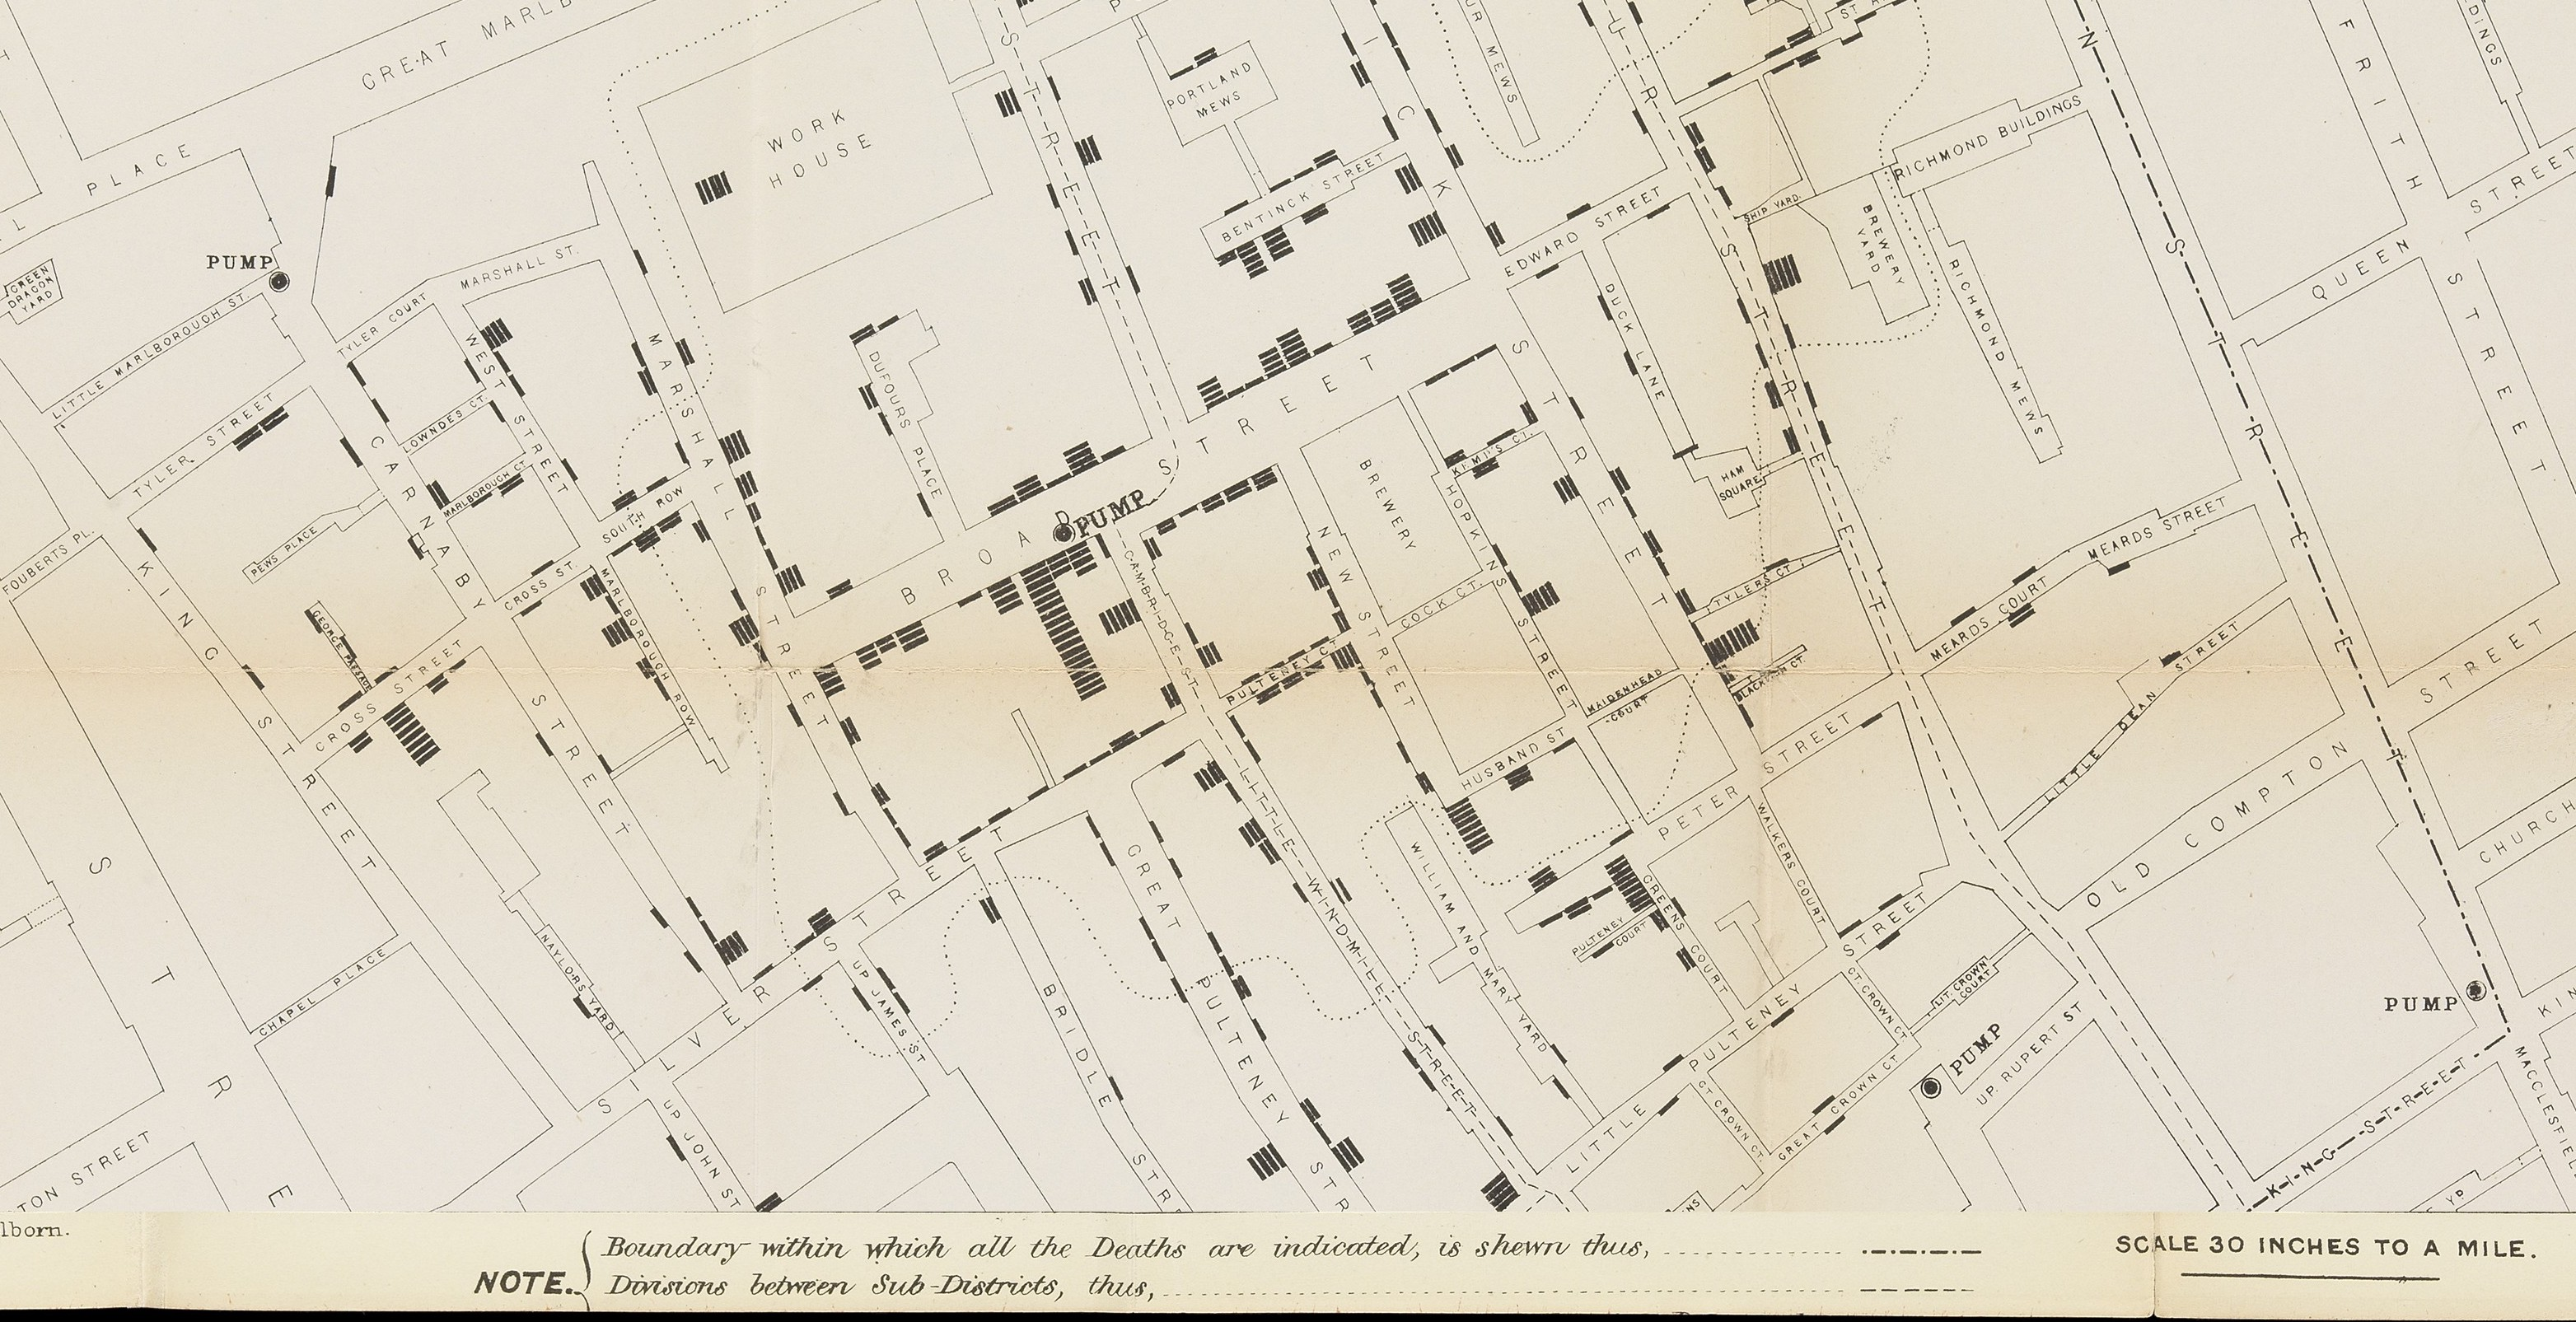
\includegraphics[width = \textwidth]{figures/snow_map_edited}\\
Source: \href{https://commons.wikimedia.org/wiki/File:A_map_taken_from_a_report_by_Dr._John_Snow_Wellcome_L0072917.jpg}{Wikimedia Commons}
\end{frame}

\begin{frame}{Hern\'an (2016): Does Water Kill?}
Does drinking \only<3->{\only<3-3>{\bblue{a swig of}}\only<4->{a swig of} }\only<2->{\only<2-2>{\bblue{fresh}}\only<3->{fresh} }water \only<4->{\only<4-4>{\bblue{from the Broad Street pump}}\only<5->{from the Broad Street pump} }\only<5->{\only<5-5>{\bblue{between August 31 and September 10}}\only<6->{between August 31 and September 10} }\only<7->{\only<7-7>{\bblue{and not initiating a rehydration treatment if diarrhea starts}}\only<8->{and not initiating a rehydration treatment if diarrhea starts} }kill\only<1-5>{?} \vskip .5cm
\only<6->{\only<6-6>{\bblue{compared with drinking all your water from other pumps?}}\only<7->{compared with drinking all your water from other pumps?}} \vskip .8cm
\onslide<9->{
\begin{center}
\large The \bblue{definition} of the causal effect is unclear without details. \vskip .4cm 
}
\onslide<10->{
\bblue{Recommendation:} Specify versions\\``until no meaningful vagueness remains,''\\\citep{hernan2016}
}
\end{center}
\end{frame}

\begin{frame}
\Large \centering
But some vagueness is \vskip .3cm
{\LARGE \bblue{unavoidable}} \vskip .3cm
in both \bgreen{experimental} and \bgreen{observational}\\social science.
\end{frame}

\begin{frame}
\centering
\begin{tikzpicture}[x = .5\textwidth, y = .45\textheight]
\node (a2) at (-.7, 0) {$A$};
\node (d2) at (0, 0) {$D$};
\node (x2) at (0, .3) {$U$};
\node (y2) at (.7, 0) {$Y$};
\draw[->, thick] (a2) -- (d2);
\draw[->, thick] (d2) -- (y2);
\draw[->, thick] (x2) -- (d2);
\node[align = center] (t2) at (-.7, .3) {Target\\population};
\draw[<->, thick] (t2.east) to[bend left = 20] (x2.west);
\node[anchor = north, align = center] at (a2.south) {Push\\notification\\sent};
\node[anchor = north, align = center] at (d2.south) {iPhone push received\\Android push received\\No push received};
\node[anchor = north, align = center] at (y2.south) {Takes\\10-minute\\walk};
\end{tikzpicture}
\end{frame}


\exampleSlideObservational{
\only<1-1>{
\fill[white] (-.01,0) rectangle (1,1.15);
}
\only<1-2>{
\fill[white] (-1.1,-1) rectangle (1,0.05);
}
\only<1-3>{
\fill[white] (0.05,-1) rectangle (1,0);
}
\only<4-4>{}
}
%\exampleSlideExperimental

\mytc{-1}{0}{white}
\section{Formalizing the Problem}
\label{sec:problem}
\mytc{-1}{0}{blue}

\subsection{Potential Outcomes}
\label{sec:potentialOutcomes}
\mytc{-2}{1}{blue}

\begin{frame}
\begin{center}
\begin{tikzpicture}[y = 1cm,x = 1.3cm]
\node[font = \Large] at (0,0) {Causal effect = $Y_i(a^\prime) - Y_i(a)$};
\node[olive, font = \small] at (1.2,-1) {Potential outcomes};
\draw[->, thick, olive] (.8, -.7) -- (.6, -.35);
\draw[->, thick, olive] (1.6, -.7) -- (1.8, -.35);
\end{tikzpicture} \vskip .4cm
\begin{tikzpicture}[x = .5\textwidth]
\node[font = \Large] at (-.5,0) {$\underbrace{\left\{Y_i(a)\right\}}_{\substack{\text{Potential outcomes:}\\\text{\bblue{Deterministic} consequence of $a$}}}$};
\node[font = \Large] at (.5, 0) {$\underbrace{Y_i^\text{Obseved} = Y_i(A_i)}_{\substack{\text{Observed outcome:}\\\text{\bblue{Random} because $A_i$ is random}}}$};
\end{tikzpicture}
\end{center}
\citet[p. 10]{imbens2015}:
\begin{quote}\normalfont
\dots for each unit, there are no different forms or versions of each treatment level which lead to different potential outcomes.
\end{quote}
\end{frame}

\begin{frame}
\begin{center}
\begin{tikzpicture}[x = 1.5in, y = 1in]
\node (a) at (0,0) {$A$};
\node (d) at (1,0) {$D$};
\node (y) at (2,0) {$Y$};
\node[anchor = north] at (a.south) {Push notification};
\node[anchor = north, align = center] at (d.south) {iPhone push received\\Android push received\\No push received};
\node[anchor = north, align = center] at (y.south) {Walks\\10 minutes};
\draw[->, thick] (a) -- (d);
\draw[->, thick] (d) -- (y);
\end{tikzpicture}
\end{center} \vspace{-.5cm}
$Y_i(a)$ is deterministic under either:
\begin{itemize}
\item Deterministic detailed treatment assignment $D$ given $A$
$$\P(D_i=d\mid A_i=a) = \begin{cases}
1 & \text{for one value of $d$} \\
0 & \text{for all other values of $d$}
\end{cases}\qquad \forall a$$
\item Treatment variation irrelevance \begin{footnotesize}(adapted from \citealt{vanderweele2009})\end{footnotesize}
$$Y_i(d) = Y_i(d^\prime) \hspace{5pt} \forall \hspace{5pt} \{d,d^\prime\} \text{ such that}$$
$$\P(D_i=d\mid A_i = a)>0 \text{ and } \P(D_i=d^\prime\mid A_i = a)>0$$
\end{itemize}
\end{frame}

\mytc{-2}{1}{blue}
\subsection{Stochastic Counterfactuals}
\label{sec:stochasticCounterfactuals}
\mytc{-3}{1}{blue}

\begin{frame}%{Stochastic counterfactuals: $Y_i(a)$ is random}
\bblue{Stochastic counterfactuals}\footnote{\citealt{vanderweele2009}, \citealt{imbens2015} p. 12} allow a more plausible assumption of treatment variation irrelevance. \vskip .4cm
Under \bblue{\only<1-1>{fixed}\only<2-2>{stochastic}} counterfactuals \vskip .2cm
Treatment-variation irrelevance:
$$Y_i(a,d_a) \blue{\only<1-1>{=}\only<2-2>{\stackrel{D}{\sim}}} Y_i(a,d_a^\prime) \quad \forall \quad \{d_a,d_a^\prime\}\in\mathcal{D}_a$$
Thus can define $Y_i(a)\blue{\only<1-1>{\equiv}\only<2-2>{\sim}} Y_i(a,d_a)$ for any $d_a$.\vskip .4cm
Consistency:
$$\text{If }A_i=a, \quad \exists \hspace{5pt} d_a\in\mathcal{D}_a\text{ such that }Y_i^\text{Observed} = Y_i(a,d_a)$$
\end{frame}


\mytc{-3}{1}{blue}
\subsection{Causal Graphs}
\label{sec:causalGraphs}
\mytc{-4}{1}{blue}

\begin{frame}
\centering
In causal graphs, the absence of hidden versions is a\\\bblue{theorem} rather than an \bblue{assumption} \citep{pearl2010}. \pause
%Consistency is a \bblue{theorem} rather than an \bblue{assumption}\\in causal graphs \citep{pearl2010}. 
\vskip 1cm
Treatment effects are defined by the DAG.\vskip 1cm \pause
A correct DAG \bblue{implies} a well-defined effect.
%\begin{tikzpicture}[x = .5\textwidth]
%\node at (-1,0) {};
%\node at (1,0) {};
%\node[anchor = east, align = center] (a) at (-.25,0) {A correct\\DAG};
%\node[anchor = west, align = center] (b) at (.25,0) {A well-defined\\effect};
%\draw[->, line width = 2pt, blue] (a) node[midway, above]{\bblue{Implies}} -- (b);
%\end{tikzpicture}
\end{frame}


\begin{frame}
\begin{tikzpicture}[x = .5\textwidth, y = .3\textheight]
\node at (-1,-1) {};
\node at (1,1) {};
\node (y) at (.5, .5) {Death};
\node[align = center] (d) at (-.5, .5) {Swallowed from the\\Broad Street pump};
\draw[->, line width = 2pt, blue] (d) -- (y);
\node[align = center] (london) at (-.5,0) {Lives in London};
\node[align = center] (date) at (.5, 0) {Date};
\draw[->, thick] (date) -- (y);
%\node[align = center] (rehydration) at (.5, .1) {Rehydration};
%\draw[->, thick] (d) -- (rehydration);
\draw[->, thick] (london) -- (d);
\draw[->, thick] (london) to[out = 0, in = 210] (y);
\onslide<2-4>{
\node[align = center] (a) at (-.5, 2.1) {Went to\\Broad Street pump};
\node[align = center] (a2) at (-.5, 1.65) {Pumped handle};
\node[align = center] (a3) at (-.5, 1.3) {Water exited at velocity $v$};
\node[align = center] (a4) at (-.5, .95) {Raised cup to mouth};
\draw[->, thick] (a) -- (a2);
\draw[->, thick] (a2) -- (a3);
\draw[->, thick] (a3) -- (a4);
\draw[->, thick] (a4) -- (d);
}
\onslide<3-3>{
\draw[->, line width = 1.5pt, red] (a) to[out = 0, in = 90] node[midway, above = 4pt, font = \bf]{?} (y);
\draw[->, line width = 1.5pt, red] (a2) to[out = 0, in = 90] (y);
\draw[->, line width = 1.5pt, red] (a3) to[out = 0, in = 90] (y);
\draw[->, line width = 1.5pt, red] (a4) to[out = 0, in = 90] (y);
}
\onslide<6-6>{
\node[align = center] (r) at (0.1,1) {Rehydration\\therapy};
\draw[->, line width = 2pt, blue] (d) -- (r);
\draw[->, line width = 2pt, blue] (r) -- (y);
}
\onslide<8-8>{
\node[align = left, anchor = north] at (0, 2) {$\begin{aligned}
	&\E\left(\text{Death}\mid \substack{
		\doop(\text{Swallowed from Broad Street pump}),\\
		\text{Living in London on August 31 -- September 10}
	}\right) \\
	&-\E\left(\text{Death}\mid \substack{
		\doop(\text{Did not swallow from Broad Street pump}),\\
		\text{Living in London on August 31 -- September 10}
	}\right)
	\end{aligned}$};
}
\onslide<9->{
\node[draw = red, line width = 2pt, rounded corners,align=center, font = \large] at (0,1.5) {Things are vague only if the \bred{graph} is insufficiently precise\\(and thus wrong).};
}
\end{tikzpicture}
\end{frame}

\begin{frame}
\begin{tikzpicture}[x = .5\textwidth, y = .45\textheight]
\node at (-1,-1) {};
\node at (1,1) {};
\node[text width = \textwidth] at (0,.8) {\bblue{Consistency}: $Y_i^\text{Observed} = Y_i(a_i)$. Is this an assumption?};
\onslide<2->{
\node[text width = \textwidth] at (0,.4) {\citet{hernan2016}: Potential death $Y$ under weight $a$ depends on whether weight is set by smoking or by moderate exercise.};
}
\onslide<3->{
\node[align=center] at (0,0) {But we could just label these as confounding variables.\\Not clear that consistency is an assumption.};
\node[align = center] (d) at (-.25, -.6) {Weight};
\node (y) at (.25, -.6) {Death};
\draw[->, line width = 2pt, blue] (d) -- (y);
\node[align = center] (smoking) at (-.25,-.3) {Smoking};
\node[align = center] (exercise) at (-.25, -.9) {Moderate exercise};
\draw[->, thick] (smoking) -- (d);
\draw[->, thick] (exercise) -- (d);
\draw[->, thick] (smoking) -- (y);
\draw[->, thick] (exercise) -- (y);
}
\end{tikzpicture}
\end{frame}

\mytc{-4}{1}{blue}
\section{When It Matters}
\label{sec:consequences}
\mytc{-5.5}{0}{blue}

\subsection{Experiments}
\label{sec:experiments}
\mytc{-6.5}{1}{blue}

\begin{frame}
\large \centering
Experiments identify causal effects with minimal assumptions,\vskip .2cm
but they often seek to generalize to a \bblue{target population}. \vskip .5cm \pause
Versions of treatment make generalization difficult.\\
{\small\citep{hernan2011}}
\end{frame}

\begin{frame}
\centering
If there is \bgreen{contextual variation} in $A\rightarrow Y$, then the effect may not generalize to new contexts.\vskip .2cm
\onslide<2->{
	If this arises from variation in $A\rightarrow D$, then measuring $D$ may promote transportability of inference.
}
\begin{tikzpicture}[x = 1.1in, y = .6in]
\node at (-1,-1.9) {};
\node at (3,1.5) {};
\node (a) at (0,0) {$A$};
\node (y) at (2,0) {$Y$};
\only<1-1>{
	\node (u) at (2,.6) {Context};
}
\only<2-2>{
	\node (u) at (1,.6) {Context};
}
\only<3-4>{
	\node at (1,-1.7) {$A\rightarrow Y$ may differ across hospitals};
	\node[anchor = north] at (a.south) {Surgery};
	\node[anchor = north] at (y.south) {Survival};
	\only<3>{
		\node (u) at (2,.6) {Hospital};
	}
	\only<4>{
		\node (u) at (1,.6) {Hospital};
		\node[anchor = north,align=center] at (d.south) {Surgeon};
	}
}
\only<5-6>{
	\node at (1,-1.7) {$A\rightarrow Y$ may differ by time of day};
	\node[anchor = north,align=center] at (a.south) {Randomized to\\restaurant ad\\on Facebook};
	\node[anchor = north,align=center] at (y.south) {Clicks\\on ad};
	\only<5>{
		\node (u) at (2,.6) {Time of day};
	}
	\only<6>{
		\node (u) at (1,.6) {Time of day};
		\node[anchor = north,align=center] at (d.south) {Ad appears\\below posts\\about dinner};
	}
}
\only<7-8>{
	\node at (1,-1.7) {$A\rightarrow Y$ may differ by rates of compliance};
	\node[anchor = north,align=center] at (a.south) {Given\\aspirin};
	\node[anchor = north,align=center] at (y.south) {Headache\\gone};
	\only<7>{
		\node (u) at (2,.6) {Complier};
	}
	\only<8>{
		\node (u) at (1,.6) {Complier};
		\node[anchor = north,align=center] at (d.south) {Takes\\Aspirin};
	}
}
\only<1,3,5,7>{
	\draw[->, thick] (a) -- (y);
	\draw[->, thick] (u) -- (y);
}
\only<2,4,6,8>{
	\node (d) at (1,0) {$D$};
	\draw[->, thick] (a) -- (d);
	\draw[->, thick] (d) -- (y);
	\draw[->, thick] (u) -- (d);
}
\end{tikzpicture}
\end{frame}

\exampleSlideExperimental


\mytc{-6.5}{1}{blue}

\subsection{Observational studies}
\label{sec:observational}
\mytc{-7.5}{1}{blue}
\exampleSlideObservational

\subsubsection{Effects may be an unusual average}
\label{sec:unusualAverage}
\mytc{-8.5}{1.2}{blue}

\begin{frame}
\begin{center}
\begin{tikzpicture}[x = .5\textwidth, y = .3\textheight]
\node (d) at (-.25,0) {$D$};
\node (y) at (.25,0) {$Y$};
\draw[->, line width = 2pt, blue] (d) -- (y);
\end{tikzpicture}
\end{center}
Because the collapsed $\mathcal{C}(D)$ is not in the causal graph, the effect of a collapsed treatment is undefined. \pause We might examine:\\{\footnotesize (\citet[Prop. 8]{vanderweele2013}, though notation differs.)}
\begin{align*}
&\E(Y\mid \mathcal{C}(D) = c) = \sum_{d \in \mathcal{C}^{-1}(c)}
		\E\big(Y\mid \doop(D = d)\big)
		\P\big(D = d\mid D \in \mathcal{C}^{-1}(c)\big)
\end{align*} \vspace{-.3cm}
\begin{center}
\pause
\bblue{\underline{One causal contrast}} \vskip .2cm
\begin{tikzpicture}[x = .5\textwidth, y = .45\textheight]
\node at (0, .35) {$\E(Y\mid \mathcal{C}(D) = c^\prime) - \E(Y\mid \mathcal{C}(D) = c)$};
\pause
\node[align=center, font = \footnotesize] at (-.5, 0) {Observed detailed treaments $d$\\mapping to collapsed treatment $c^\prime$};
\draw[rounded corners] (-.95, -.2) rectangle (-.05, .2);
\pause
\node[align=center, font = \footnotesize] at (.5, 0) {Observed detailed treaments $d$\\mapping to collapsed treatment $c$};
\draw[rounded corners] (.95, -.2) rectangle (.05, .2);
\pause
\node[font = \footnotesize] (drawPrime) at (-.5, -.35) {Random draw};
\draw[->, line width = 2pt, gray] (-.5,-.16) -- (drawPrime);
\pause
\node[font = \footnotesize] (draw) at (.5, -.35) {Random draw};
\draw[->, line width = 2pt, gray] (.5,-.16) -- (draw);
\pause
\node[font = \footnotesize] (difference) at (0, -.35) {Difference};
\draw[->, line width = 2pt, gray] (draw) -- (difference);
\draw[->, line width = 2pt, gray] (drawPrime) -- (difference);
\pause
\node[font = \footnotesize] (average) at (0, -.55) {Average over many reps};
\draw[->, line width = 2pt, gray] (difference) -- (average);
\end{tikzpicture}
\end{center}
\end{frame}

\begin{frame}
\begin{center}
\begin{tikzpicture}[x = .5\textwidth, y = .3\textheight]
\node[anchor = east, align = right] at (-.4, 0) {With covariates. {\footnotesize (equivalent to }\\{\footnotesize \citealt[Prop. 8]{vanderweele2013})}};
\node[draw, outer sep = -3pt] (x) at (-.3,0) {$X_j$\hspace{6pt}{}};
\node (d) at (0,0) {$D$};
\node (y) at (.3,0) {$Y$};
\draw[->, thick] (x) -- (d);
\draw[->, thick] (x) to[bend left = 20pt] (y);
\draw[->, line width = 2pt, blue] (d) -- (y);
%\onslide<2-2>{
%\node[align = center, text width = .8\textwidth, draw = red, line width = 2pt, rounded corners, fill = white] at (0,0) {Comparisons between $c^\prime$ and $c$ average over \bred{different shifts} in $D$ in different cells of $\vec{X}$.};
%}
\end{tikzpicture}
\end{center} \vspace{-.5cm}
\begin{align*}
&\E(Y\mid \mathcal{C}(D) = c, \vec{X} = \vec{x}) = \\
&\quad \sum_{d \in \mathcal{C}^{-1}(c)}
		\E\big(Y\mid \doop(D = d), \vec{X} = \vec{x}\big)
		\P\big(D = d\mid D \in \mathcal{C}^{-1}(c), \vec{X} = \vec{x}\big)
\end{align*}
\begin{center} \vspace{-.3cm}
\bblue{\underline{One causal contrast}} \\
\begin{tikzpicture}[x = .5\textwidth, y = .45\textheight]
\pause
\node at (0, .4) {$\sum_{\vec{x}}\P(\vec{X} = \vec{x})\bigg(\E(Y\mid \mathcal{C}(D) = c^\prime, \vec{X} = \vec{x}) - \E(Y\mid \mathcal{C}(D) = c, \vec{X} = \vec{x})\bigg)$};
\pause
\draw[rounded corners, gray, line width = 2pt] (-1, -.65) rectangle (1, .25);
\node[anchor = south east, font = \footnotesize] at (1,-.65) {among $\vec{X} = \vec{x}$};
\pause
\node[align=center, font = \footnotesize] at (-.5, 0) {Observed detailed treaments $d$\\mapping to collapsed treatment $c^\prime$};
\draw[rounded corners] (-.95, -.2) rectangle (-.05, .2);
\pause
\node[align=center, font = \footnotesize] at (.5, 0) {Observed detailed treaments $d$\\mapping to collapsed treatment $c$};
\draw[rounded corners] (.95, -.2) rectangle (.05, .2);
\pause
\node[font = \footnotesize] (drawPrime) at (-.5, -.35) {Random draw};
\draw[->, line width = 2pt, gray] (-.5,-.16) -- (drawPrime);
\pause
\node[font = \footnotesize] (draw) at (.5, -.35) {Random draw};
\draw[->, line width = 2pt, gray] (.5,-.16) -- (draw);
\pause
\node[font = \footnotesize] (difference) at (0, -.35) {Difference};
\draw[->, line width = 2pt, gray] (draw) -- (difference);
\draw[->, line width = 2pt, gray] (drawPrime) -- (difference);
\pause
\node[font = \footnotesize] (average) at (0, -.55) {Average over many reps};
\draw[->, line width = 2pt, gray] (difference) -- (average);
\pause
\node[font = \footnotesize] (average2) at (0, -.75) {Average over $\vec{X}$};
\draw[->, line width = 2pt, gray] (0,-.6) -- (0,-.72);
\end{tikzpicture}
\end{center}
\end{frame}

\mytc{-8.5}{1.2}{blue}
\subsubsection{Heterogeneous treatment effects may really be the effects of heterogeneous treatments}
\label{sec:heterogeneousEffects}
\mytc{-9.5}{1.2}{blue}

\begin{frame}
\centering
\begin{tikzpicture}[x = .5\textwidth, y = .3\textheight]
\node at (-1, -1) {};
\node at (1, 1) {};
\node[align = center, text width = \textwidth] at (0,.8) {What is the effect of \bblue{overwork} ($>$ 50 hours) on the \bblue{hourly wage} of those working at least 40 hours per week?\\Suppose \bblue{gender} is the only source of confounding.};
\onslide<2->{
\node (d) at (0,0) {Employment hours};
\node at (0,-.3) {$\text{Overwork} = \mathcal{C}(\text{Employment hours}) = \mathbb{I}(\text{Hours} > 50)$};
\node (y) at (.8,0) {Hourly wage};
\node (x) at (-.8,0) {Gender};
\draw[->, thick] (x) to[bend left = 20] (y);
\draw[->, thick] (x) -- (d);
\draw[->, thick] (d) -- (y);
}
\onslide<3->{
\node[align = left, font = \small] at (0,-.7) {$\E\big(\text{Wage}\mid \doop(\text{Overwork}), \text{Man}\big) = \sum_{h > 50}
		\bigg(\substack{
			\only<3-4,6->{
				\E\big(\text{Wage}\mid \doop(\text{Hours} = h), \text{Man}\big)
			}\only<5>{
				\blue{\E\big(\text{Wage}\mid \doop(\text{Hours} = h), \text{Man}\big)}
			}\\
			\only<3-5,7->{
				\times\P\big(\text{Hours} = h\mid \text{Hours}>50, \text{Man}\big)
			}
			\only<6>{
				\times\blue{\P\big(\text{Hours} = h\mid \text{Hours}>50, \text{Man}\big)}
			}
		}$\bigg)};
}
\onslide<4->{
\node[align = left, font = \small] at (0,-1.2) {$\E\big(\text{Wage}\mid \doop(\text{Overwork}), \text{Woman}\big) = \sum_{h > 50}
		\bigg(\substack{
			\only<3-4,6->{
				\E\big(\text{Wage}\mid \doop(\text{Hours} = h), \text{Woman}\big)
			}\only<5>{
				\blue{\E\big(\text{Wage}\mid \doop(\text{Hours} = h), \text{Woman}\big)}
			}\\\only<3-5,7->{
				\times\P\big(\text{Hours} = h\mid \text{Hours}>50, \text{Woman}\big)
			}\only<6>{
				\blue{\times\P\big(\text{Hours} = h\mid \text{Hours}>50, \text{Woman}\big)}
			}
		}$\bigg)};
}
\onslide<5-5>{
	\node[blue, font = \small] at (-.5,-1.6) {Heterogeneous treatment effects};
}
\onslide<6-6>{
	\node[blue, font = \small] at (0.2,-1.6) {Effects of heterogeneous treatments};
}
\end{tikzpicture}
\end{frame}

\mytc{-9.5}{1.2}{blue}
\section{What To Do}
\label{sec:recommendations}
\mytc{-12}{0}{blue}

\begin{frame}{What To Do}
In randomized \bblue{experiments} aiming to generalize:
\begin{itemize}
\item Randomize a detailed treatment
\item Theorize context-specific versions likely to remain
\end{itemize}
In \bblue{observational} studies:
\begin{itemize}
\item Estimate at the finest level of detail measured
\begin{itemize}
\item[---] Promotes a simple definition of the effect
\item[---] Promotes transportability
\item[---] Promotes clear policy implications
\end{itemize}
\item If treatment remains vague, state the implied intervention.
\end{itemize}
\end{frame}

\mytc{-1}{0}{white}

\appendix

\begin{frame}
\huge \centering Appendix
\end{frame}

\begin{frame}
Some define the \bblue{assumptions} for causal inference as:\vskip .3cm
\begin{itemize}
\setlength\itemsep{.3cm}
\item Ignorable treatment assignment
\begin{itemize}
\item[---] Violated if the treated would do better even without treatment
\end{itemize}
\item Positivity
\begin{itemize}
\item[---] Violated if $\P(\text{Treated})$ is 0 or 1 for some units
\end{itemize}
\item Stable Unit Treatment Value Assumption
\begin{itemize}
\item[---] Violated if there is interference
\item[---] Violated if there are hidden versions of treatment
\end{itemize}
\end{itemize} \vskip .2cm
In this setup, \bblue{hidden versions} are the second part of SUTVA. Social scientists often focus on the first assumptions and give less thought to this part of SUTVA.
\end{frame}

\begin{frame}{Why not use the $Y(a,d_a)$ notation?}
One could state potential outcomes as a function of both treatment and treatment version \citep{vanderweele2009,hernan2011,vanderweele2013}. \vskip .2cm
\begin{center}
\bblue{Versions of treatment}\vskip .2cm
\begin{tikzpicture}[x = 1in, y = .5in]
\node (a) at (0,0) {$A$};
\node (d) at (1,0) {$D$};
\node (y) at (2,0) {$Y$};
\draw[->, thick] (a) -- (d);
\draw[->, thick] (d) -- (y);
\end{tikzpicture}
\end{center}
$Y_i(a,d_a)$ is unnecessary notation, though. Because only one $a$ exists for any given $d$, $Y_i(d)$ carries the same information.\\ In contrast, this is useful in mediation.
\begin{center}
\bblue{Mediation}\vskip .2cm
\begin{tikzpicture}[x = 1in, y = .5in]
\node (a) at (0,0) {$A$};
\node (m) at (1,.5) {$M$};
\node (y) at (2,0) {$Y$};
\draw[->, thick] (a) -- (m);
\draw[->, thick] (m) -- (y);
\draw[->, thick] (a) -- (y);
\end{tikzpicture}
\end{center}
$Y_i(a,m)$ is valuable. Because $A$ is not fixed given $M$, there exist multiple $\{a,a^\prime\}$ with $Y_i(a,m)\neq Y_i(a^\prime,m)$.
\end{frame}

\begin{frame}{Why not put $A$ on the DAG as a consequence of $D$?}
When the researchers take a detailed treatment $D$ and coarsen it into an aggregate treatment $A$, \citet{hernan2011} put it in the DAG as a consequence of $D$.
\begin{center}
\begin{tikzpicture}[x = 1in, y = .5in]
\node (d) at (0,0) {$D$};
\node (a) at (1,0) {$A$};
\node (y) at (2,0) {$Y$};
\draw[->, thick] (d) -- (a);
\draw[->, thick] (d) to[bend left] (y);
\end{tikzpicture}
\end{center}
The reasons not to do this are
\begin{enumerate}
\item In a DAG, it is useful to be able to conceive of an intervention to any given node. Because $D\rightarrow A$ is deterministic, it is hard to imagine an intervention to $A$ which has no consequence for $D$. By the DAG, this intervention would have no consequence for $D$. This seems hard to swallow.
\item Perhaps $A$ is not deterministic: it is \emph{reported} $D$. But this seems like a whole different set of issues, and it is clear even without the DAG that intervening to change a report would have no consequence for $Y$.
\end{enumerate}
\end{frame}

\begin{frame}{What about when $A\rightarrow D$ is confounded?}
When treatment precedes version, \citet{hernan2011} also include cases like below:
\begin{center}
\begin{tikzpicture}[x = 1in, y = .5in]
\node (u) at (0,1) {$U$};
\node (a) at (0,0) {$A$};
\node (d) at (1,0) {$D$};
\node (y) at (2,0) {$Y$};
\draw[->, thick] (u) -- (a);
\draw[->, thick] (u) -- (d);
\draw[->, thick] (a) -- (d);
\draw[->, thick] (d) -- (y);
\end{tikzpicture}
\end{center}
The reasons not to do this are
\begin{enumerate}
\item The edge $U\rightarrow A$ implies this is an observational study rather than an experiment. In observational studies, I usually do not believe the story that $A$ is assigned first, followed by $D$. I think in observational studies $D$ is typically the only variable involved.
\item We already have transportability issues from $U\rightarrow D$ alone. Omitting $U\rightarrow A$ helps to highlight these problems in the scenario when $A$ is randomized.
\end{enumerate}
\end{frame}

\begin{frame}{References}
\bibliography{collapsed_treatments.bib}
\end{frame}

\end{document}